% -------------- PREAMBULO ------------ %
\documentclass[a4paper, 12pt]{report}
\usepackage[left = 3cm, top = 2.5cm, bottom = 3cm, right = 2.5cm]{geometry}
\usepackage[spanish]{babel}
\usepackage[utf8]{inputenc}  %Uso de simbolos directamente del teclado
\usepackage[T1]{fontenc}     %Salida 
\usepackage{graphicx}        %Manejo de figuras y graficos

\usepackage{booktabs}        %Para formar tablas
\usepackage{longtable, multirow}        %Para formar tablas largas y multicolumnas
\usepackage{color}           %Para usar colores
\usepackage{setspace}        %Usado para doble espacio, espacio y medio y espacio simple (\onehalfspace  \doublespacing  \singlespace)
\usepackage{ragged2e}
\usepackage{times}			 %Tipo de letra
\usepackage{anyfontsize}     %PErmite usar modificar los tamaños de letra
\usepackage{titlesec}	     %Modificar el titulo
\setcounter{secnumdepth}{3}  %Para que ponga 1.1.1.1 en subsubsecciones
\setcounter{tocdepth}{3}     %Para que ponga subsubsecciones en el indice
\bibliographystyle{apalike}  %Bibliografía Norma APA
\usepackage{natbib}
%                            Crear colores                      %     
\definecolor{rosaclaro}{RGB}{247,180,180}

%                            redefiniendo comandos              %
\renewcommand{\chaptername}{\bf{\large{\underline{CAP\'ITULO}}}}
\titleformat{\chapter}[display]{\normalfont}{\bf\large\filcenter\large\ \underline{CAP\'ITULO \thechapter}}{0.5em}{\large\bfseries\filcenter\underline}
\renewcommand{\tablename}{Tabla} 
% -------------- CUERPO ------------ %
\begin{document}
%%%%%%%%%%%%%%%%%%%%%%%%%%%% PORTADA %%%%%%%%%%%%%%%%%%%%%%%%%%%%
\pagestyle{empty}                          
\spacing{1.2}

\begin{center}
 {\bf {\fontsize{18}{20.8}\selectfont UNIVERSIDAD NACIONAL DE TRUJILLO}}  
  
 {\bf{\fontsize{16}{18.8}\selectfont Facultad de Ciencias Físicas y Matemáticas}} 
 
 {\bf{\fontsize{16}{18.8}\selectfont Escuela Académico Profesional de Informática}} 	
\end{center}  

\vskip .5cm
\begin{figure}[ht]
	\begin{center}
		\includegraphics[width=.3\textwidth]{unt}
	\end{center}
\end{figure}

\begin{center}
	{\bf {\fontsize{18}{20.4}\selectfont{Monograf\'ia que como parte del curso de T\'opicos en Procesamiento Paralelo:}}}
	
	{\bf {\fontsize{19}{20.4}\selectfont{\vskip .2cm ``Estado del Arte de Cloud Computing''}}}
\end{center}   

\vskip 1.5cm
{\bf {\fontsize{17}{20.4}\selectfont{Nombre de autor(es):}}} 

\begin{center}
	\fontsize{14}{16.8}\selectfont{\'Alvarez Carbajal, Gaby Yuri}		
	
	\fontsize{14}{16.8}\selectfont{Cruz Leyva, Segundo Junior}
	
	\fontsize{14}{16.8}\selectfont{Gonza Llaque, Renato Fabrizzio}
	
	\fontsize{14}{16.8}\selectfont{Guevara Liz\'arraga, Mar\'ia Fernanda}
	
	\fontsize{14}{16.8}\selectfont{Lavado Azabache, Jonatan E....}
\end{center}

{\bf {\fontsize{17}{20.4}\selectfont{Nombre del Asesor:\vskip .5cm}}} 
\begin{center}  
{\fontsize{14}{14}\selectfont{Mg. Mendoza, Edwin}}
\end{center}  

\vskip 3cm
\begin{center}    
	{\bf {\fontsize{14}{16.8}\selectfont Trujillo - La Libertad
	\\ 2016 }}
\end{center} 
\newpage
%%%%%%%%%%%%%%%%%%%%%%%%%%%%%%%%%%%%%%%%%%%%%%%%%%%%%%%%%%%%%%%%%%%%%%%%%%%
\pagestyle{plain}
\doublespacing
\pagenumbering{Roman}
%%%%%%%%%%%%%%%%%%%%%%%%%%%% RESUMEN %%%%%%%%%%%%%%%%%%%%%%%%%%%%
\addcontentsline{toc}{chapter}{Resumen}
\vspace*{6em}
\begin{center}
{\bf{\large{\underline{RESUMEN}}}}
\end{center}
\begin{justify}
Holaque hace como esta muy bien esxop me legr qurbfgs tu vida hace triempo bla bla bla bla bla xd xd xd d
\end{justify}
\newpage
%%%%%%%%%%%%%%%%%%%%%%%%%%%%%%%%%%%%%%%%%%%%%%%%%%%%%%%%%%%%%%%%%%%%%%%%%%%



%%%%%%%%%%%%%%%%%%%%%%%%%%%% INTRODCUCCION %%%%%%%%%%%%%%%%%%%%%%%%%%%%
\addcontentsline{toc}{chapter}{Introducción}
\vspace*{6em}
\begin{center}
{\bf{\large{\underline{INTRODUCCI\'ON}}}}
\end{center}
\begin{justify}
Holaque hace como esta muy bien esxop me legr qurbfgs tu vida hace triempo bla bla bla bla bla xd xd xd d
\end{justify}
\newpage
%%%%%%%%%%%%%%%%%%%%%%%%%%%%%%%%%%%%%%%%%%%%%%%%%%%%%%%%%%%%%%%%%%%%%%%%%%%


\singlespacing
%%%%%%%%%%%%%%%%%%%%%%%%%%%% INDICEs %%%%%%%%%%%%%%%%%%%%%%%%%%%%\\
\renewcommand{\contentsname}{\centering\bf{\large{{\'INDICE GENERAL}}}}
\renewcommand{\listfigurename}{\centering\bf{\large{{LISTA DE FIGURAS}}}}
\renewcommand{\listtablename}{\centering\bf{\large{{LISTA DE TABLAS}}}}

\tableofcontents    % indice de materias
\addcontentsline{toc}{chapter}{\'Indice General}
\listoffigures      % indice de figuras
\addcontentsline{toc}{chapter}{Lista de Figuras}
\listoftables       % indice de tablas
\addcontentsline{toc}{chapter}{Lista de Tablas}

%%%%%%%%%%%%%%%%%%%%%%%%%%%%%%%%%%%%%%%%%%%%%%%%%%%%%%%%%%%%%%%%%%%%%%%%%%%
\doublespacing
%%%%%%%%%%%%%%%%%%%%%%%%%%%% CAPITULOS %%%%%%%%%%%%%%%%%%%%%%%%%%%%
%%%%%%%%%%%%%%%%%%%%%%%%%%%% CAPITULO 1 %%%%%%%%%%%%%%%%%%%%%%%%%%%%
\vspace*{5em}
\chapter{TITULO DEL CAPITULO 1}\label{cap1}
\pagestyle{plain}
\pagenumbering{arabic}
\vspace*{-2em}
\begin{justify}
Holaque hace como esta muy bien esxop me legr qurbfgs tu vida hace triempo bla bla bla bla bla xd xd xd d
\end{justify}

%%%%%%%%%%%%%%%%%%%%%%%%%%%% CAPITULO 2 %%%%%%%%%%%%%%%%%%%%%%%%%%%%
\vspace*{5em}
\chapter{TITULO DEL CAPITULO 2}
\vspace*{-2em}
\begin{justify}
Holaque hace como esta muy bien esxop me legr qurbfgs tu vida hace triempo bla bla bla bla bla xd xd xd d
\end{justify}

%%%%%%%%%%%%%%%%%%%%%%%%%%%% CAPITULO 3 %%%%%%%%%%%%%%%%%%%%%%%%%%%%
\vspace*{5em}
\chapter{TITULO DEL CAPITULO 3}
\vspace*{-2em}
\begin{justify}
Holaque hace como esta muy bien esxop me legr qurbfgs tu vida hace triempo bla bla bla bla bla xd xd xd d
\end{justify}

%%%%%%%%%%%%%%%%%%%%%%%%%%%% CAPITULO 4 %%%%%%%%%%%%%%%%%%%%%%%%%%%%
\vspace*{5em}
\chapter{TECNOLOG\'IAS ACTUALES}
\vspace*{-2em}

\par Claramente la nube se est\'a convirtiendo en una plataforma de innovaci\'on y transformaci\'on general.
\par Actualmente muchas empresas de todo el mundo est\'an ofreciendo una amplia gama de servicios en la nube, la abundancia puede ser abrumadora.
 
\section{Empresas que brindan servicios de Cloud}
\subsection{Amazon.com}
\begin{justify}
{\bf{Amazon Web Services (AWS)}} es una plataforma de servicios en la nube que ofrece potencia de c\'omputo, almacenamiento de bases de datos, entrega de contenido y otra funcionalidad para ayudar a las empresas a escalar y crecer. \citep{aws}

AWS se encuentra detrás del \'exito de muchas compañías, startups y sector p\'ublico, como: 
\begin{itemize}
	\item  \textbf{Netflix:} AWS permite a Netflix desplegar rápidamente miles de servidores y terabytes de almacenamiento en cuesti\'on de minutos. Los usuarios pueden ver programas y películas de Netflix desde cualquier parte del mundo, incluso en la web, en tabletas o en dispositivos móviles como el iPhone.\citep{awscasos}
	\item  \textbf{Spotify:}	Debido a que el objetivo de la compañía es ayudar a la gente a escuchar cualquier música que quieran, cuando quieran, Spotify se enfrenta al desaf\'io de catalogar no sólo ayer y las canciones populares de hoy, sino también todas las que se publicarán en el futuro. Spotify agrega más de 20.000 pistas al día a su catálogo. \\	
La  compa\~{n}\'ia cre\'o sistemas basados en Python para interactuar con su enorme volumen de contenido en Amazon S3. Además, Amazon CloudFront entrega la aplicación Spotify y las actualizaciones de software a los usuarios. \\ Al igual que las tendencias musicales cambian continuamente, Amazon Web Services (AWS) ayuda a Spotify a evaluar continuamente su infraestructura para cumplir con los objetivos de negocio en constante evoluci\'in.\citep{awscasos}
	\item  \textbf{Adobe:}Adobe utiliza AWS para proporcionar ambientes operativos de varios terabytes para sus clientes. Al integrar sus sistemas con AWS Cloud, Adobe puede centrarse en implementar y operar su propio software en lugar de infraestructura.\citep{awscasos}
\end{itemize}
De acuerdo con \cite{awscasos} otras  de las empresas que cuentan con el respaldo de AWS son  Dunkin Donuts, Airbnb, Kellogs, Siemens, BCP, Johmson-Johmson, etc. 
\\Actualmente la nube de AWS funciona en 44 zonas de disponibilidad dentro de 16 regiones geogr\'aficas del mundo, con planes anunciados para crear 14 zonas m\'as y cinco regiones adicionales en China, Francia, Hong Kong, Suecia y una segunda regi\'on AWS GovCloud en los EE.UU. \citep{aws}

\begin{figure}[ht]
\begin{center}
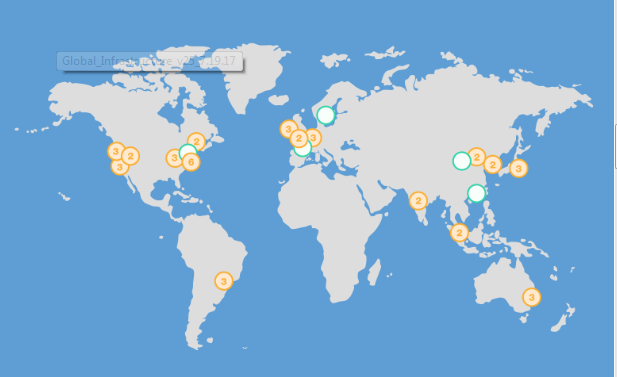
\includegraphics[scale=0.8]{aws_paises}
\end{center}
\begin{center}
\vskip -0.5cm
\caption{\small{Distribución de AWS.}}
{\small{Fuente: \cite{aws}}}
\end{center}
\end{figure}

\end{justify}
\subsection{Google Inc}
\begin{justify}
{\bf Google Cloud Plataform} consiste en un conjunto de servidores d f\'isico as\'i como virtuales que est\'an contenidos en los centros de datos de Google alderedor del mundo.
\\ Google cuenta con el modo de despliegue  multi regional Google Cloud Plataform, lo cual permite al usuario elegir el centro de datos para sus aplicaciones.
\end{justify}
\begin{figure}[ht]
\begin{center}
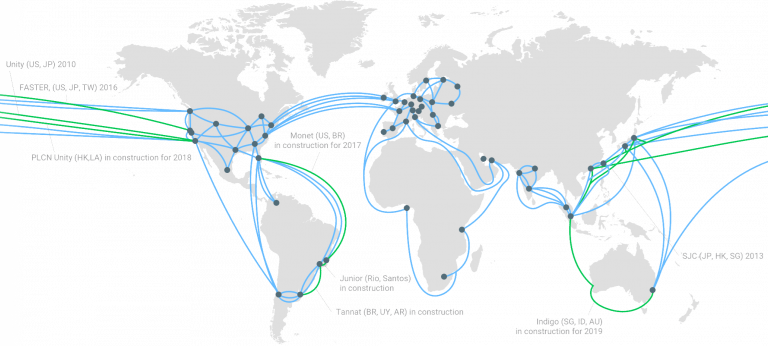
\includegraphics[scale=0.6]{google_cloud}
\end{center}
\begin{center}
\vskip -0.5cm
\caption{\small{Red de Google Cloud Platform.}}
{\small{Fuente: \cite{google_cloud}}}
\end{center}
\end{figure}
\begin{justify}
Según \cite{google_cloud} en las \'ultimas encuestas de SADA Systems sobre el uso p\'ublico de la nube, los  gerentes de TI encuestados dan se\~{n}ales del crecimiento que esta teniendo hoy en día la insfraestructura de nube p\'ublica.
\end{justify}
\begin{figure}[ht]
\begin{center}
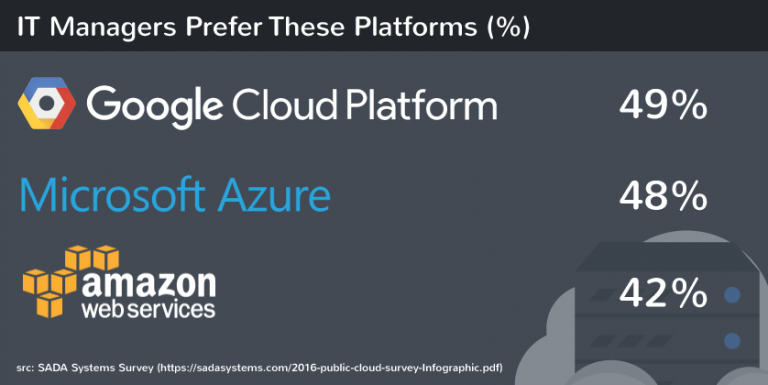
\includegraphics[scale=0.4]{encuesta}
\end{center}
\begin{center}
\vskip -0.5cm
\caption{\small{Resultados de Encuesta sobre el uso de nubes p\'ublicas}}
{\small{Fuente: \cite{google_cloud}}}
\end{center}
\end{figure}

Estas son algunas de las empresas que  desarrollan sus productos con Google Cloud Platform:
\begin{itemize}
	\item \textbf{Pocket Gems:} Utiliza App Engine para procesar cientos de miles de jugadores móviles en tiempo real.
	\item \textbf{Khan Academy :}Khan Academy usa Google Cloud Platform para poner cursos gratuitos y de gran calidad al alcance de todos.
	\item \textbf{Coca-Cola:} Comprueba cómo está utilizando Google Cloud Platform Coca-Cola para estar a la altura de los eventos deportivos más grandes del mundo.
	\item \textbf{Atomic Fiction:} Crea efectos especiales para las series de televisión y las películas más importantes del mundo, gracias a los potentísimos recursos informáticos de Google Cloud Platform.
\end{itemize}
\begin{justify}
Un gran punto a favor que tiene hoy en día Google Cloud Plataform es que permite la migraci\'on en vivo de m\'aquinas Virtuales, funcionalidad que ni Azure ni AWS tienen. En la siguiente figura se detallan los  pasos de alto nivel involucrados en una migración de VM en vivo (Figura \ref{migracion}).
\end{justify}
\begin{figure}[h!]\label{migracion}
\begin{center}
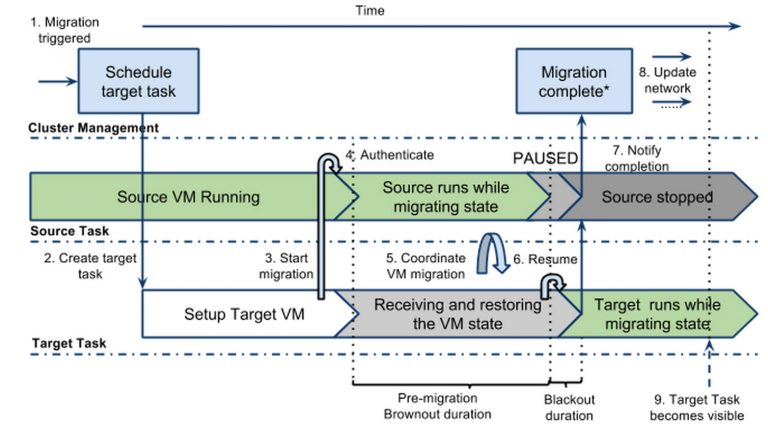
\includegraphics[scale=0.7]{migracion}
\end{center}
\begin{center}
\vskip -0.5cm
\caption{\small{ Pasos de alto nivel involucrados en una migraci\'on de VM en vivo}}
{\small{Fuente: \cite{google_cloud_migration}}}
\end{center}
\end{figure}

\subsection{Azure}
\begin{justify}
Microsoft Azure es una creciente colección de servicios en la nube integrados que los desarrolladores y los profesionales de TI utilizan para crear, implementar y administrar aplicaciones a través de nuestra red global de centros de datos. Con Azure, obtiene la libertad de crear e implementar donde quiera, utilizando las herramientas, las aplicaciones y los marcos que prefiera.\citep{azure_def}

Estas son algunas de las empresas que  desarrollan sus productos con Microsoft Azure:
\begin{itemize}
	\item \textbf{Carviresa :} Para mejorar la planificación y gestión de sus recursos, y centralizar los datos de negocio procedentes de sus tres ubicaciones.
	\item \textbf{Guzman Global :}La multinacional española ha elegido Microsoft Dynamics CRM Online por su usabilidad, escalabilidad y sus altos estándares de seguridad en la nube, factores que le permiten replicar su modelo fácilmente en diferentes países.
	\item \textbf{NAE :} Para mejorar su gestión comercial con la ayuda del partner Innovar Tecnologías.
\end{itemize}

\end{justify}

\section{Casos de Implementación}
	\begin{justify}
	A continuación se presentarán  las diferentes que empresas o instituci\'on que aplicaron las buenas pr\'acticas en la implementaci\'on de diferentes soluciones cloud (Tabla \ref{tablaEmpresas}) , casos pertenecientes a diferentes ramas, actividad económica, administración publica, etc.
	\end{justify}

	\begin{table}%%%[h]
		\label{tablaEmpresas}
		\centering
		\caption{Casos de \'Exito implementando Cloud Computing}
		\begin{tabular}{|p{4.2cm} |p{2.3cm} |p{2.5cm} |p{4cm}|} \hline
			\bf{Sector} & \bf{Proveedor} & \bf{Modelo de Negocio} & \bf{Empresa o Institución} 
			\\ \hline \hline
			Adminitraci\'on P\'ublica & Microsoft & SaaS &  Generalitat de Catalunya 
			\\ \cline{2-4}
			 & CIPSA y REGTSA & SaaS (cloud privada) & CIPSA y REGTSA  
			\\ \hline
			Audio Visuales  & Spotify & SaaS & AWS
			\\ \hline
			Correo electr\'onico & Amazon & PaaS / IaasS & AWS
			\\ \hline
			Inform\'atica y telecomunicaciones & Annova y Pixelware & PaaS & Proyecto PymeCloud 
			\\ \cline{2-4}
			 & EyeOS & PaaS & EyeOS  
			\\ \cline{2-4}
			 & Arsys & SaaS / PaaS / IaaS & EyeOS  
			\\  \cline{2-4}
			 & Fresh Books & SaaS & Fresh Books  
			\\  \hline
			Ivestigaci\'on, desarrollo y manufactura & Windows Azure & PaaS & 3M 
			\\ \hline
			Ivestigaci\'on Biom\'edica & VORTAL & SaaS & Organismo P\'ublico de España 
			\\ \hline
			Medios de Comuniaci\'on & NTS y Salesforce.com & SaaS & Grupo Vocento \\ \hline
			Transporte & Estudio Cero & SaaS & Estudio Cero\\ \hline 
		\end{tabular}
		\vskip 0.2cm
		\begin{center}
			{\small{Fuente: Elaboraci\'on Propia - \cite{Ferrari}.}}
		\end{center}
	\end{table}



\section{Diferencias entre Empresas que ofrecen Cloud Computing}
	\begin{justify}
	Seg\'un \cite{Akami} las empresas de Cloud Computing se diferencian seg\'un:
	\begin{itemize}
		\item \textbf{Tipo de servicio ofrecido: } En la nube existen diferentes tipos de servicio (v\'ease cap. \ref{cap1}. La entidad que se quiera contratar debe definir muy bien cu\'ales ser\'an los Acuerdos de Nivel de Servicio (SLA) que mejor se ajusten a las necesidades.
		\item \textbf{La escala y resistencia de la arquitectura:} Las mejores empresas de cloud computing tienen varios centros de datos dispersos geográficamente, lo que garantiza la disponibilidad ininterrumpida del servicio para sus cliente.
		\item \textbf{Calidad del componente de autoservicio:} La administraci\'on  de los servicios en la nube se realiza por un portal web, por ello, el portal debe contar con ciertas normas y permitir el control f\'acil del servicio.
		\item \textbf{Longevidad y experiencia:} Seg\'un \cite{CristianCA} en el 2012  el modelo de cloud computing se encontraba en etapa de desarrollo, por ese motivo existían pocas empresas que apostaban por el modelo; sin embargo,  en la actualidad existen cada día mas empresas ofreciendo este modelo, este es el motivo por el que cual al momento de querer adquirir los servicios que ofrece se debe tener en cuenta la experiencia, pues muchas son nuevas y no han sido probadas.
	\end{itemize}
	Si desea conocer algunas recomendaciones para contratar servicios en la nube revise el documento de \cite{Beimar}
\end{justify}


%%%%%%%%%%%%%%%%%%%%%%%%%%%%%%%%%%%%%%%%%%%%%%%%%%%%%%%%%%%%%%%%%%%%%%%%%%%


\newpage
%%%%%%%%%%%%%%%%%%%%%%%%%%%% CONCLUSIONES %%%%%%%%%%%%%%%%%%%%%%%%%%%%
\addcontentsline{toc}{chapter}{Conclusiones}
\vspace*{6em}
\begin{center}
{\bf{\large{\underline{CONCLUSIONES}}}}
\end{center}
\begin{justify}
Holaque hace como esta muy bien esxop me legr qurbfgs tu vida hace triempo bla bla bla bla bla xd xd xd d bla bla blan
\end{justify}
%%%%%%%%%%%%%%%%%%%%%%%%%%%%%%%%%%%%%%%%%%%%%%%%%%%%%%%%%%%%%%%%%%%%%%%%%%%



%%%%%%%%%%%%%%%%%%%%%%%%%%%% BIBLIOGRAFIA %%%%%%%%%%%%%%%%%%%%%%%%%%%%
\addcontentsline{toc}{chapter}{Bibliograf\'ia}
\vspace*{6em}
 \bibliography{Bibliografia}
%%%%%%%%%%%%%%%%%%%%%%%%%%%%%%%%%%%%%%%%%%%%%%%%%%%%%%%%%%%%%%%%%%%%%%%%%%%



\end{document}
